% !TEX TS-program = pdflatex
% !TeX program = pdflatex
% !TEX encoding = UTF-8
% !TeX spellcheck = en_US

\documentclass{../../../extra/aakpract/aakpract}

\usepackage{wrapfig}

\settitle{BERT from scratch}
\setversion{Lab04}
\setyear{2024-2025}
\setauthor{Mr. Abdelkrime Aries}


\begin{document}

\maketitle

\begin{center}
	\begin{minipage}{0.8\textwidth}
		\small
		We aim to implement a BERT encoder from scratch in order to deepen our understanding of how Transformer architectures function. 
		This project also serves as an opportunity to practice designing a clean and minimal Python API following open-source principles. 
		Note that this implementation will focus solely on the encoder and will not include pretraining heads such as the masked language model or next sentence prediction.
	\end{minipage}
\end{center}

\section{Implementation}

In this lab, we aim to implement a simple Python API, which we will refer to as "\textbf{mybert}" for clarity. 
The project structure is illustrated in Figure \ref{fig:mybert}, where each package corresponds to a Python module (i.e., a file). 
At the root of the project, the \_\_init\_\_.py file defines a common interface named Module, which is implemented by two abstract base classes: Layer and Model.
All module types must implement two core methods:
\begin{itemize}
	\item \textbf{forward}: Computes and returns the output of the module based on the input and any internal parameters. It may also store intermediate values required for the backward pass.
	\item \textbf{backward}: Takes a gradient vector (matching the shape of the output) and a learning rate, updates the internal parameters accordingly, and returns the gradient with respect to the input—allowing gradient flow to previous layers.
\end{itemize}

In our design, Layer and Model are structurally similar. 
However, "Model" is intended to include additional functionality such as model saving and loading.
"Layer" introduces two optional methods: forward\_single and backward\_single, which operate on individual samples (e.g., a single sentence). 
These methods are not mandatory, and you may choose to implement only the batch-oriented forward and backward methods if preferred.

\begin{figure}[htp]
	\centering
	\includegraphics[width=0.6\textwidth]{img/class_diagram.pdf}
	\caption{Class diagram of "mybert" project}
	\label{fig:mybert}
\end{figure}


\subsection{Implemented parts}


Several utility functions analogous to NumPy's have been implemented across two modules: "vec\_func" (for vector operations) and "mat\_func" (for matrix operations). 
While functionally similar, these implementations are not as optimized as NumPy's, which relies on lower-level languages like C or Rust for performance. 
As expected, the matrix module builds upon the vector module, since matrices are conceptually represented as vectors of vectors.

Another core module is "layers", which provides implementations for several essential components: SeqLinear, Embedding, LayerNorm, and ScaledDotProductAttention. 
These serve as the foundational building blocks of the project. 
Each of these layers expects input tensors with the shape (batch, sequence, features).

The "bert" module includes several helper functions:
\begin{itemize}
	\item \textbf{split\_heads}: Reshapes an input tensor of shape (batch, sequence, embedding\_size) into (num\_heads, batch, sequence, head\_size), where head\_size = embedding\_size / num\_heads.
	
	\item \textbf{merge\_heads}: Reverses the transformation applied by split\_heads.
	
	\item \textbf{construct\_mask}: Builds a 2D attention mask matrix from a 1D mask vector for each item in the batch.
	
	\item \textbf{tensor3\_ew\_add}: Performs element-wise addition of two 3-dimensional tensors.
\end{itemize}

{\footnotesize \begin{verbatim}
	def split_heads(X: List[List[float]], 
	                num_heads: int, head_dim: int) -> List[List[List[float]]]
	def merge_heads(heads: List[List[List[float]]]) -> List[List[float]]
	def construct_mask(mask: List[List[bool]]) -> List[List[List[bool]]]
	def tensor3_ew_add(X: List[List[List[float]]], Y: List[List[List[float]]]
	                    ) -> List[List[List[float]]]
\end{verbatim}}



\subsection{MultiheadAttention class}

\begin{wrapfigure}{r}{0.2\textwidth}
	\centering
	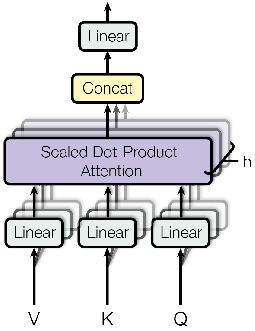
\includegraphics[width=\linewidth]{img/multi_head_att2_.pdf}
\end{wrapfigure}

In this class, we define a multi-head attention mechanism using a specified number of attention heads, $ num\_heads $, each with a dimensionality of $ head\_dim $. 
Each head independently projects the input into queries, keys, and values, all of dimension $ head\_dim $. 
These projections are then processed using the scaled dot-product attention mechanism. 
The resulting output vectors from all heads are concatenated and passed through a final linear layer to produce the output projection.

In our implementation, we use three linear layers (for keys, queries, and values), each with input and output dimensions equal to $dim\_model$. 
After computing the projections, we split them across the attention heads. 
To apply attention, we instantiate one attention object per head.
This is necessary because each attention object must retain intermediate values during the forward pass for use in the backward pass.

The backward step proceeds as follows: we first call the backward method of the final output linear layer to compute gradients with respect to its input. 
These gradients are then split across the heads. 
Next, we iterate over each head and invoke the backward method of the corresponding attention object using its respective gradient. 
This yields gradients for keys, queries, and values, which are collected into separate lists. 
Finally, the gradients for each component (keys, queries, and values) are merged across heads and passed through the backward functions of their respective linear projection layers.

\newpage
\subsection{BertBlock class}

\begin{wrapfigure}{r}{0.2\textwidth}
	\centering
	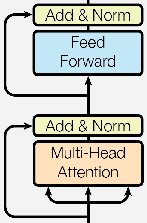
\includegraphics[width=\linewidth]{img/encoder_block_.pdf}
\end{wrapfigure}

In this layer, we apply multi-head self-attention to the input. 
Since this is part of an encoder, it uses self-attention, meaning the queries, keys, and values are all equal to the input $X$.
The attention output is then added element-wise to the input (residual connection) and passed through a first normalization layer.
The output of this normalization is then processed by a two-layer feed-forward network (FFN). 
In our case, both linear layers are implemented without bias. 
The first layer projects the input to an intermediate dimension and applies an activation function (which, for simplicity, we assume to be linear). 
The second layer projects the result back to the model's dimensionality. 
The output of the feed-forward network is then added element-wise to the output of the first normalization layer, followed by a second normalization, yielding the final output of this encoder block.

The backward pass is straightforward: we apply the backward methods of each layer in reverse order. 
If a tensor is used by multiple components (e.g., due to residual connections), the corresponding gradients are accumulated by summing them element-wise.


\subsection{Bert class}

BERT takes as input the token IDs, segment IDs, and an attention mask (see Figure~\ref{fig:mybert2}). 
The position IDs correspond to the index of each token in the sequence and can be constructed dynamically within the forward pass.
During the forward step, we generate embeddings for the tokens, segments, and positions. 
These three embeddings are then added element-wise to form a single input representation. 
This combined representation is passed through the first encoder block, whose output is then passed to the next block, and so on. 
The final output of the last encoder block serves as the model’s contextualized representation.

In the backward step, gradients are propagated from the last block back to the first. 
The gradient output from the first block is then passed into the embedding layers to compute gradients for the token, segment, and position embeddings during their respective backward passes.


\begin{figure}[htp]
	\centering
	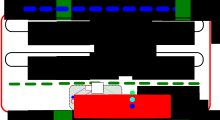
\includegraphics[width=0.8\textwidth]{img/bert-arch.pdf}
	\caption{Architecture of Bert.}
	\label{fig:mybert2}
\end{figure}


\newpage
\section{Logistics}

This lab must be completed in teams of at most \textbf{2} students.
It is designed to be completed within \textbf{1 hour and 15 minutes}, and the assignment should be submitted by the end of the session.
Although the lab has been tested in advance, an exceptional extension is granted, and the final deadline for submission is \textbf{midnight}.

\subsection{Evaluation}

\begin{itemize}
	\item Your implementation will be evaluated using the unit tests provided in \textbf{\texttt{test/bert\_u.py}} via \texttt{pytest}.
	\item Additionally, your code will be assessed through manual review to evaluate structure, clarity, and adherence to specifications.
\end{itemize}

\subsection{Submitting}

\begin{itemize}
	\item Submit only the file \textbf{\texttt{bert.py}}, and rename it to \textbf{\texttt{bert\_name1\_name2.py}} using the contributors' names.
	\item Ensure that both students' names are clearly listed inside the file as contributors.
	\item \textbf{Late submission policy:} A penalty of 2 points will be applied if submitted one day after the deadline. 
	Submissions beyond that will not be accepted.
	\item \textbf{Attendance policy:} Failure to attend the lab session will result in a deduction of 2 points.
\end{itemize}

\subsection{Grading}

Grade = Grade\_MultiheadAttention + Grade\_BertBlock + Grade\_Bert + Grade\_compliance
	\begin{itemize}
		\item \textbf{Grade\_MultiheadAttention}: (7pts) = forward (4pts) + backward (3pts)
		\item \textbf{Grade\_BertBlock}: (5pts) = forward (3pts) + backward (2pts)
		\item \textbf{Grade\_Bert}: (4pts) = forward (2pts) + backward (2pts)
		\item \textbf{Grade\_compliance}: (4pts) = Attendance (2pts) + On-time Submission (2pts)
	\end{itemize}

\begin{flushright}
	Good luck\footnote{Luck is an illusion; work hard to go faster, work smart to go further.}
\end{flushright}


\end{document}
